\documentclass[]{article}

\usepackage{listings}
\usepackage{float}
\usepackage{graphicx}

\usepackage{titling}
\newcommand{\subtitle}[1]{%
  \posttitle{%
    \par\end{center}
    \begin{center}\large#1\end{center}
    \vskip0.5em}%
}

\begin{document}

\title{Lab 3: Stopwatch}
\subtitle{CS M152A}
\author{Aman Agarwal \& Lowell Bander}

\maketitle
\tableofcontents \newpage

\section{Introduction}

In this lab, we implemented a simple stopwatch. The stopwatch counts up from 00:00 to 59:59 over the course of one hour during normal operation, then resets to 00:00. \\

Additionally, the stopwatch can be paused, manually reset, and the minutes and the seconds stopwatch can be modified individually at a rate of twice the normal rate. During such modification, the digits being modified blink to indicate their modification.

\section{Design Description}

\subsection{High Level Design}
\label{subsec:highlevel}

To design a stopwatch we used 3 main modules. The \texttt{state} module kept track of the stopwatch's state. The \texttt{clockConverter} module converted the input 100MHz clock to multiple different clocks of different frequencies. The \texttt{timer} module held the actual time.

Here is how our overall design looked like:

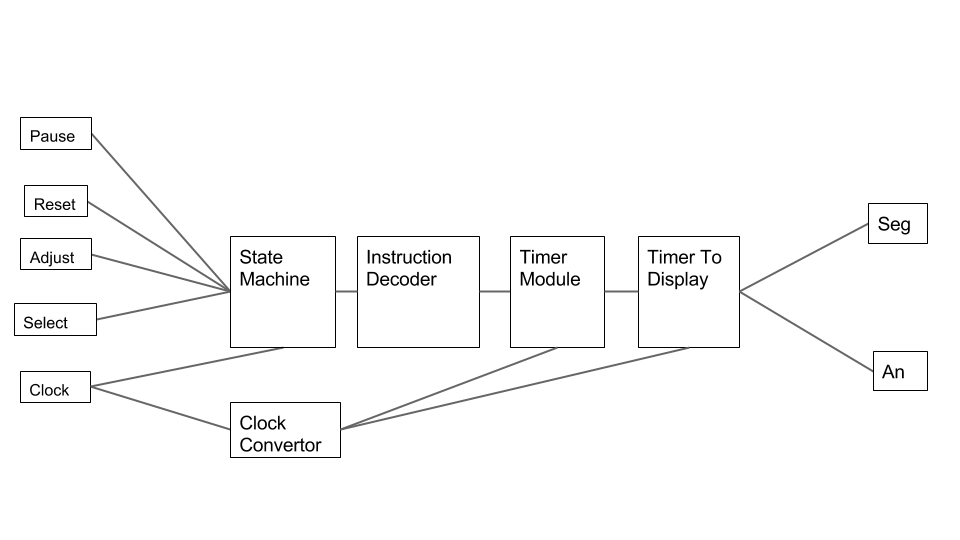
\includegraphics[width=11cm]{modularDesign.png}

\subsection{Low Level Implementation}

The source code displayed below is an a excerpt from our main module, \texttt{stopw.v}. The 3 modules described in subsection~\ref{subsec:highlevel} above are show here along with other auxilliary modules.

\lstinputlisting[language=Verilog, firstline=54, lastline=106]{stopw.v}

The \texttt{clockConverter} module created new clock signals at different frequencies by using a counter whose carry output became the new clock signal.

The state machine was a Mealy state machine that used its current state and input signals to determine its next state and output. The output was in the form of an instruction which was then decoded by the \texttt{instructionDecoder} module into signals that the \texttt{timer} module accepts. This drawing describes the state machine:

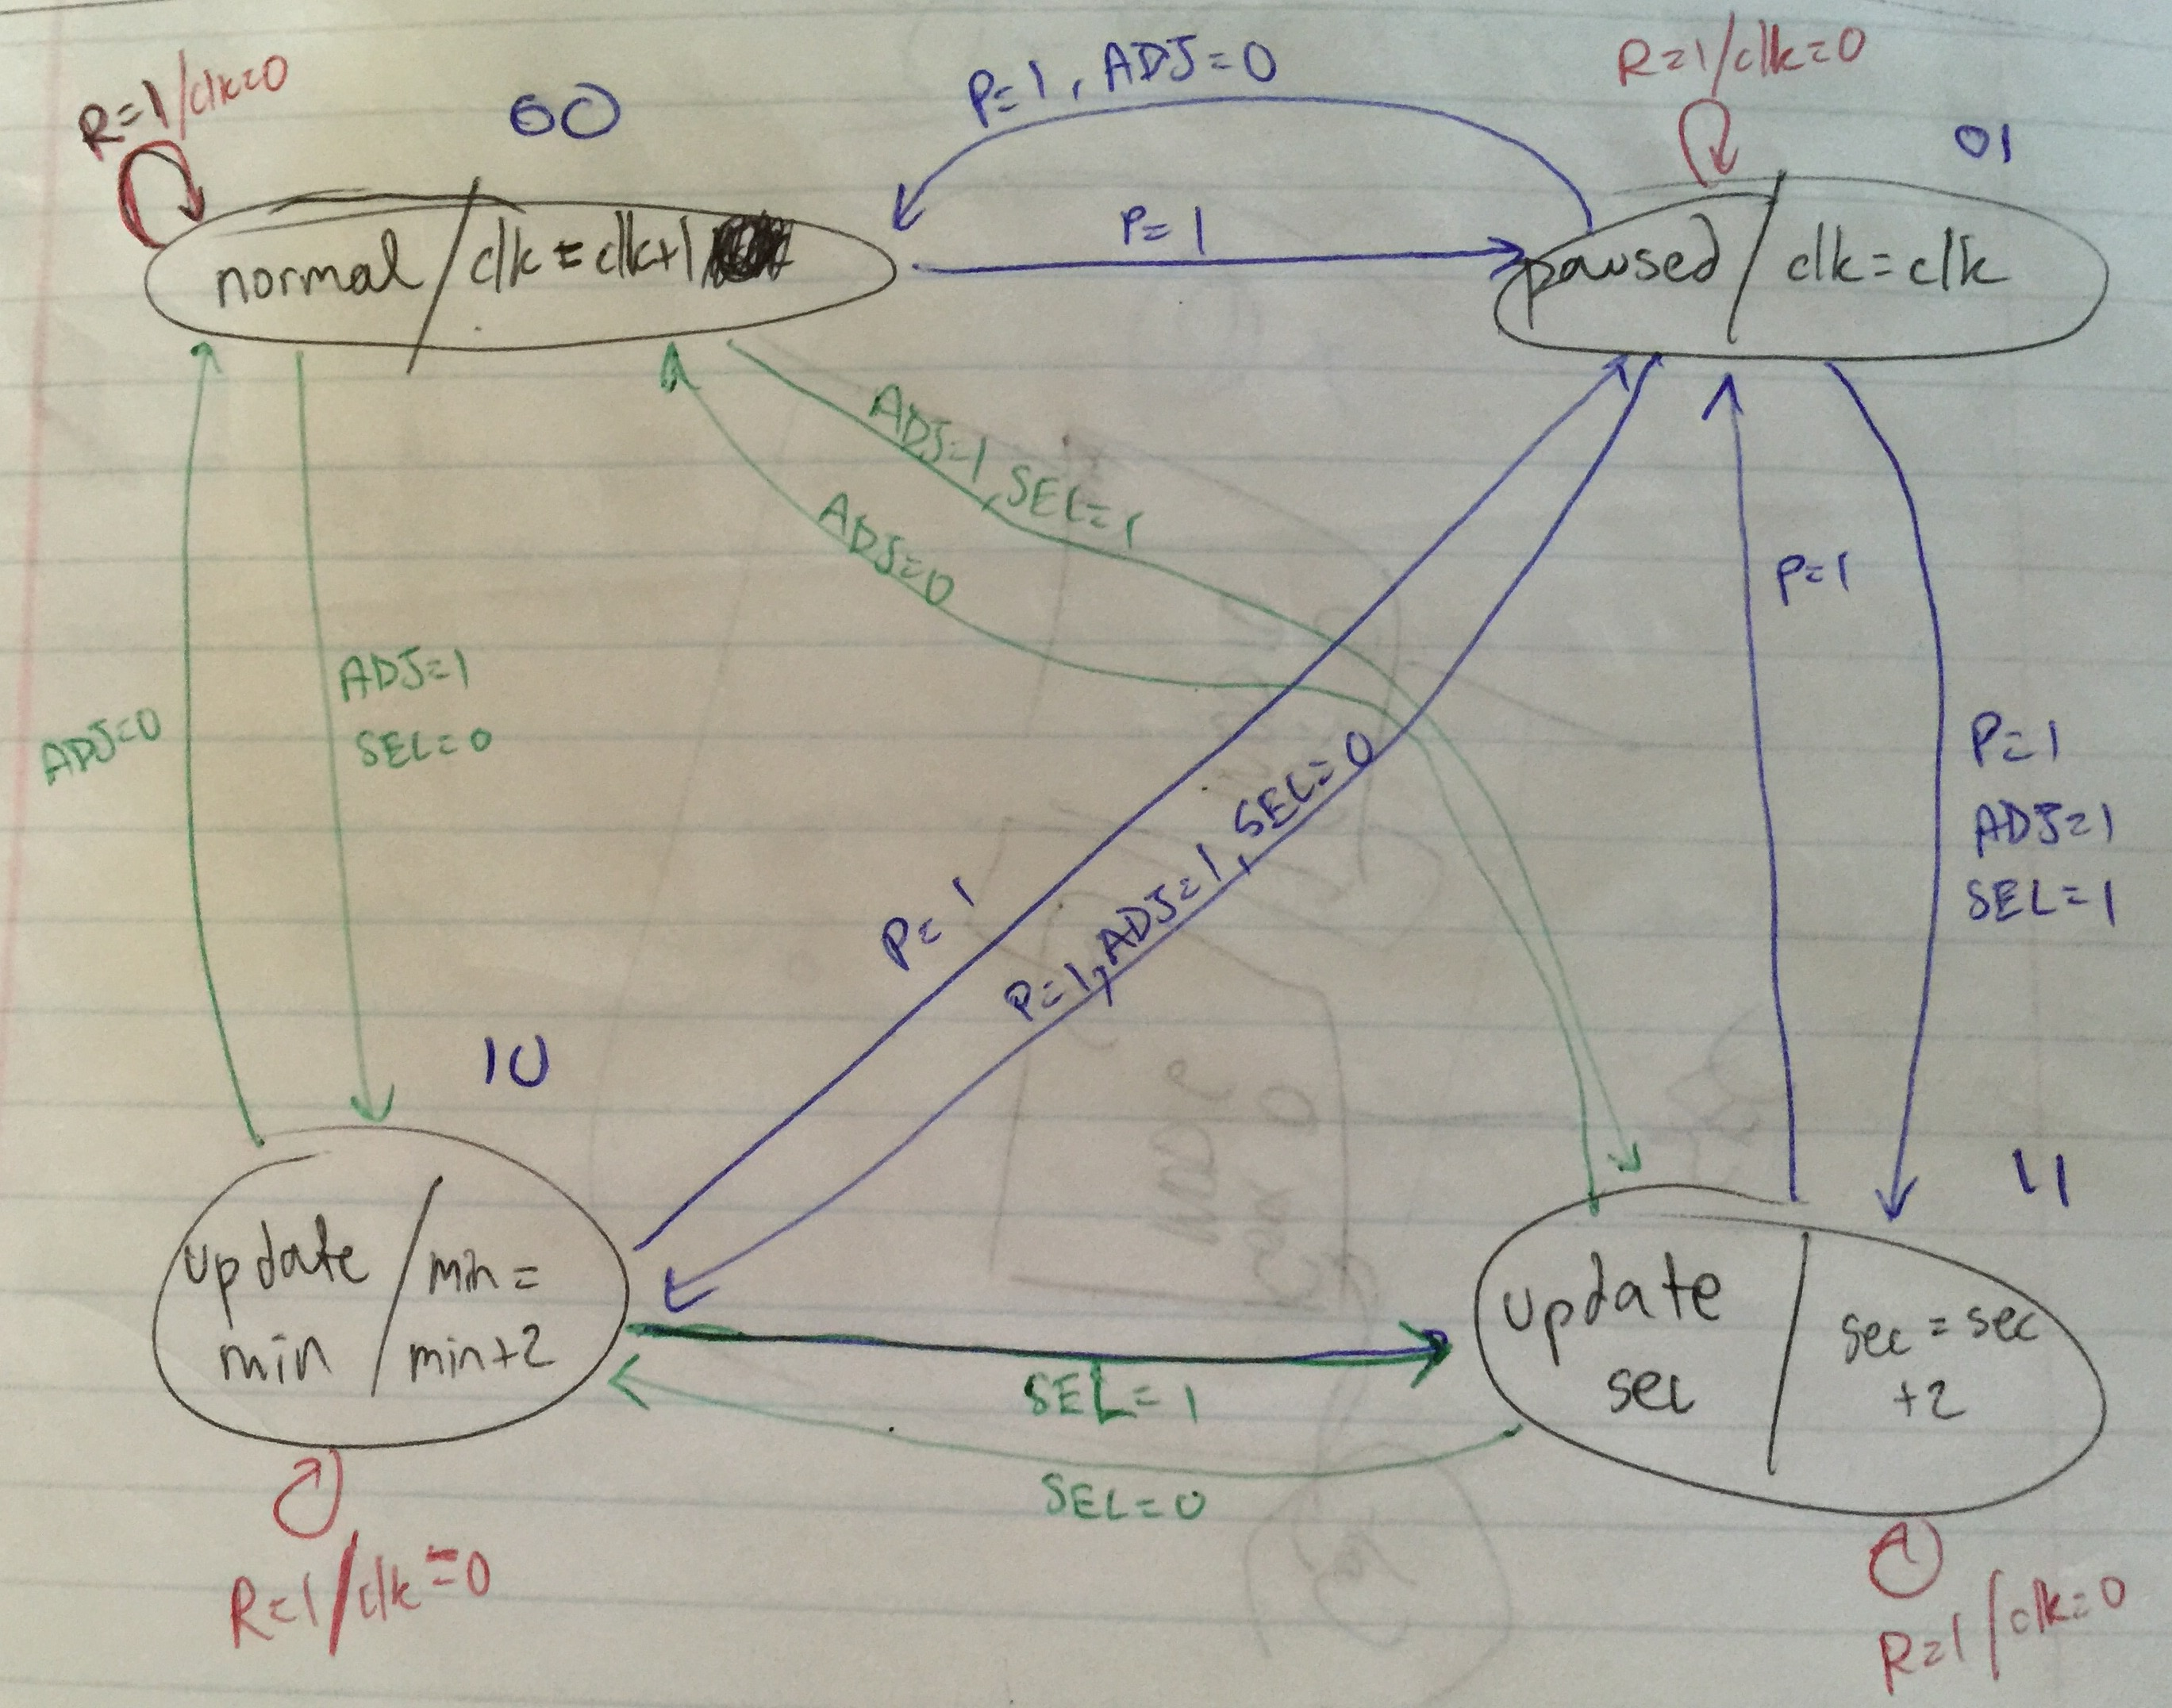
\includegraphics[width=11cm]{state_diagram.jpeg}

Along with some other modules, the \texttt{timer} module heavily relied upon counters. Because counters were so useful in this lab, we created a \texttt{CounterN} module that took as a general parameter $N$ the counter's range (from $0$ through $N - 1$).

\lstinputlisting[language=Verilog, firstline=574, lastline=603]{stopw.v}

The \texttt{timer} module kept track of the actual time and also responded to instruction sent out by the \texttt{state} module to respond to the \texttt{Adjust}, \texttt{Select}, \texttt{Pause}, and \texttt{Reset} signals. The output of the timer module was the time represented in a binary format but this was not the same as the input of the seven-segment display.

We have a \texttt{timeToDisplay} module which then took this input and converted it into the seg and an outputs for the seven-segment display. This module also takes care of flashing and cycling through each of the anodes.








\section{Simulation Documentation}

In our first labs, we made the faux pas of writing all of our code before testing any of it. This time, we developed in a very incremental and modular manner. For example, we began with a simple counter module, created a test bench for it, then chained them together to make a larger module, then tested that module, and so on. We hope this made it easy to catch issues early on in the development process.\\

In addition to testing each module as it was developed, we tested the entire device as a whole once development was complete. Namely, we tested every state transition pictured in Figure ???.\\

During simulation, we found several errors. For example, we discovered that the module which divides our clock wasn't functioning properly for one of our clocks.

\section{Conclusion}


\end{document}

